\documentclass[11pt]{article}

\usepackage{amsmath,setspace,mathtools,amssymb,booktabs,graphicx, multicol, caption}

\usepackage[utf8]{inputenc}

\usepackage[letterpaper,portrait,margin=0.5cm]{geometry}

\captionsetup{
	font = small,
	labelfont = bf,
	tableposition = top,
	belowskip = 8
}
\graphicspath{ {./} }


\title{Computational Physics Midterm}

\author{Thaseus Karkabe-Olson}

\date{}

\begin{document}
	
	
	\maketitle
	
	\begin{multicols}{2}

	\begin{center}

	\section*{Model Description}

	\end{center}

		\indent This model is set up to simulate how a number of cars n behave on a ring road given several initial conditions. These include driver reaction times,the length of vehicles, the size of the road,
		the desired speed of the drivers, and the initial positions and velocities of cars.

		\indent From this we can find out how the cars actually move. We accomplish this by calculating the rates of change for both velocity and position of each car using the differential equation
		from the IDM model. Utilizing ODEint we can then solve for our resulting velocities and positions at each point in time along a given time interval. From there, we then simply plot our positions and
		velocities of each car to see how they behave over time. Here is an example of how 50 cars behave when spaced apart evenly and with random initial velocities:


		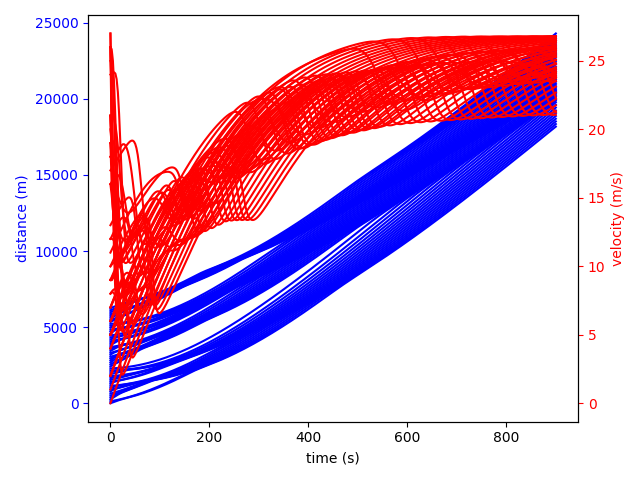
\includegraphics[scale = 0.5]{Figure_1.png}
		\captionof{figure}{An example of a complex initial setup}

		\indent You can see from this graph that we get two results: velocity and position over time for each car. Blue coorisponds to how far in total each car moves in metres, while the red coorisponds
		to what the velocity at a given time is for each car in metres per second.

	\begin{center}

	\section*{Experiments}

		\subsection*{Causes of Traffic}

	\end{center}

		\indent Here is another example of a setup, this time where all cars start at the same speed except the first and where we have a smaller road and less cars:


		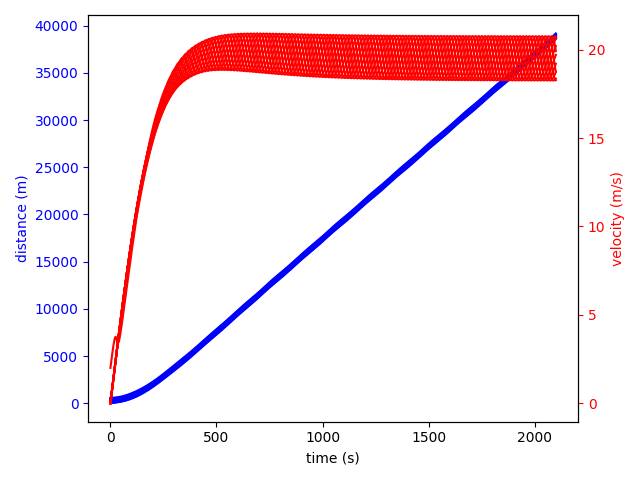
\includegraphics[scale = 0.5]{Figure_2.png}
		\captionof{figure}{Basic ring road setup $(a = 0.1, b = 2, Nc = 10)$}

		\indent We can visually see that the cars oscillate around some kind of equilibrium speed, which approaches a constant value as time goes to infinity. If we change our drivers to have a quicker acceleration time,
		our plot changes like so:

		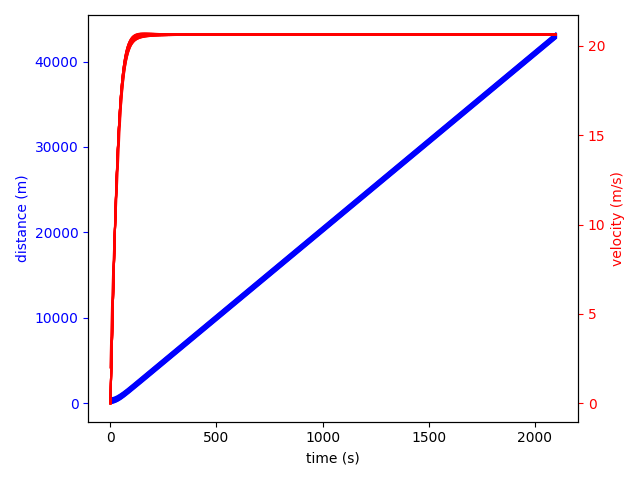
\includegraphics[scale = 0.5]{Figure_3.png}
		\captionof{figure}{Driver acceleration increased from basic setup $(a = 0.5, b = 2, Nc = 10)$}

		\indent Fundamentially this is the result that I would expect, since a faster acceleration on the part of the driver means that each driver can better react to other slowdowns, meaning that the drivers can get into
		an equilibrium state of being distanced halfway between their neighbours and stay there at their desired speed instead of continuing to have coupled motion with the other drivers. However, this greatly emphisizes
		the point that driver reaction times are one of the biggest causes of traffic. This suggests one possible solution to traffic, to be discussed later.

		\indent On the other hand, deceleration has the opposite effect, where a high deceleration value leads to drivers over committing to braking when they sense that a car is too close to them, as seen in this plot with
		a larger deceleration value:

		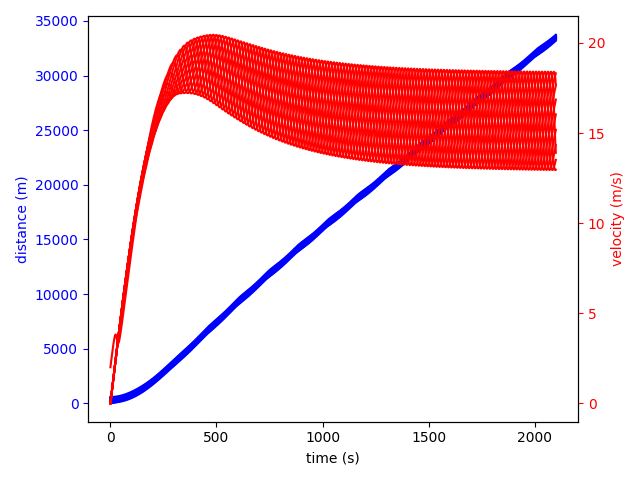
\includegraphics[scale = 0.5]{Figure_4.png}
		\captionof{figure}{Driver deceleration increased from basic setup $(a = 0.1, b = 3, Nc = 10)$}

		\indent While this likely improves safety as cars are much more jumpy and less likely to tailgate, it also kills the chance for cars to get into that ideal equilibrium state of perfect spacing and ideal speed, since
		their constant deceleration forces the cars behind them to decelerate, propagating a traffic wave.

		\indent Another major factor is the number of cars, as shown here:

		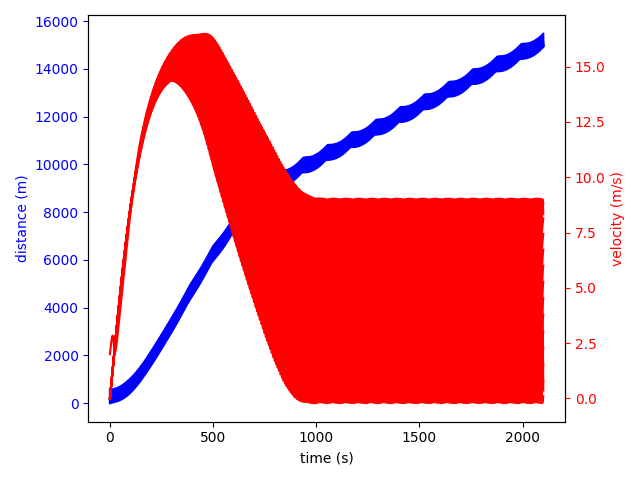
\includegraphics[scale = 0.5]{Figure_5.png}
		\captionof{figure}{Number of cars increased from basic setup $(a = 0.1, b = 2, Nc = 15)$}

		\indent In fact, this is one of the biggest factors for causing bad traffic. If 15 people need to commute in this model instead of 10, it takes a slightly unideal traffic situation and makes it stop and go instead, especially when combined with poor reaction times.

		\subsection*{Self Driving Car Solution}

			\indent One solution to traffic suggested by many is to introduce self driving vehicles that have better reaction times. This has good support from our model, where there's a clear connection between reaction times and
			traffic waves. We can clearly see in figure 3 that self driving cars appear to solve light to moderate traffic. However, we have yet to account for the type of stop and go traffic caused by a large number of cars.

			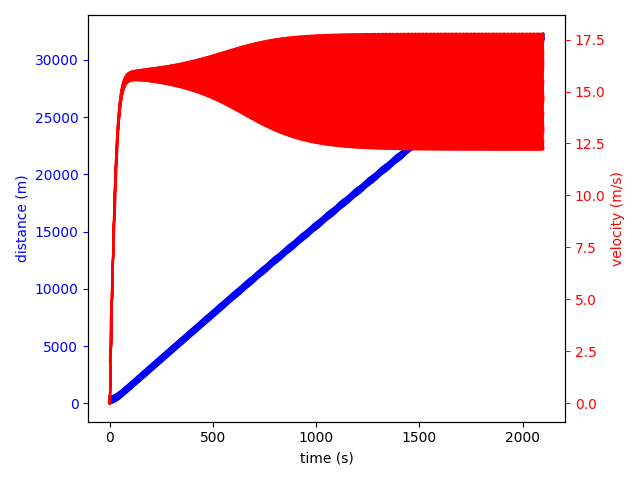
\includegraphics[scale = 0.5]{Figure_6.png}
			\captionof{figure}{More cars with better reaction times $(a = 0.5, b = 2, Nc = 15)$}

			\indent Comparing this result to result from figure 5, improving reaction times does indeed appear to be a significant improvement. Traffic is no longer stop and go, average speed is improved, and there's less varience in each
			cars speed. However, this behaviour has its limits, as seen when acceleration is made absurdly high:

			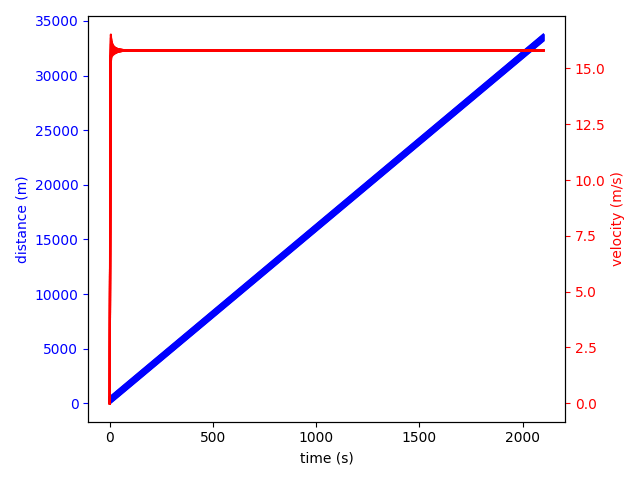
\includegraphics[scale = 0.5]{Figure_7.png}
			\captionof{figure}{More cars with near instantaneous reaction times $(a = 10, b = 2, Nc = 15)$}

			\indent This suggests one issue that can be clearly solved with better reaction times, as cars do reach an equilibrium velocity with no variation, which makes for a less frustrating overall commute. However, simply due to the number of cars we can
			immedietly see a major issue; our velocity is still capped far under the desired velocity of the drivers.

			\indent Another important issue in traffic that can be addressed with self driving cars though is safety. Here are the results of increasing reaction times both in terms of how readily the cars will break and how quickly they can accelerate:

			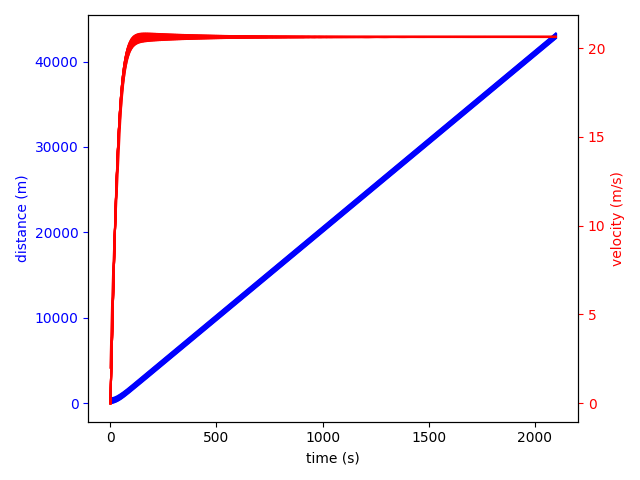
\includegraphics[scale = 0.5]{Figure_10.png}
			\captionof{figure}{Cars with generally better reaction times $(a = 0.5, b = 3, Nc = 10)$}

			\indent Here we can see that even with a much faster deceleration that our overall traffic is mostly unaffected compared to when our breaking acceleration was lower.


		\subsection*{Public Transit Solution}

			\indent Another solution to solving traffic is good public transit.To simulate adding very small busses with limited ridership to our model, I have added some vehicles with double the length, and assumed that each bus took two cars off the road. In order to
			integrate this into my model I made my length quantity an array and dispersed busses with a different length among the cars as evenly as possible. By replacing 8 cars with 4 busses, we can already see some pretty drastic results:

			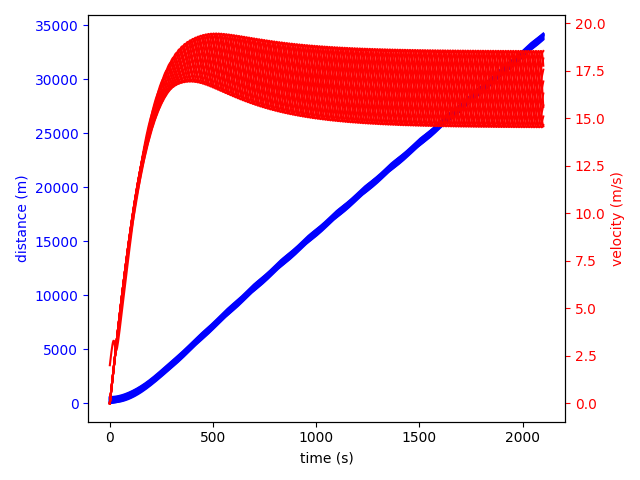
\includegraphics[scale = 0.5]{Figure_8.png}
			\captionof{figure}{More vehicles with busses $(a = 0.1, b = 2, Nc = 7, Nb = 4)$}

			\indent While there is more variation in velocity than there was with instantaneous reaction times, our overall average velocity is still higher than what we got even with instantaious reaction
			times. Comparing this to figure 5, we see an incredibly drastic improvement. In fact, our values are approaching that of having 10 cars, which perhaps shouldn't be too surprising since we have reduced the total number of vehicles on our road.

			\indent When we instead apply this solution to light/medium traffic as seen in our basic setup, we see the following results:

			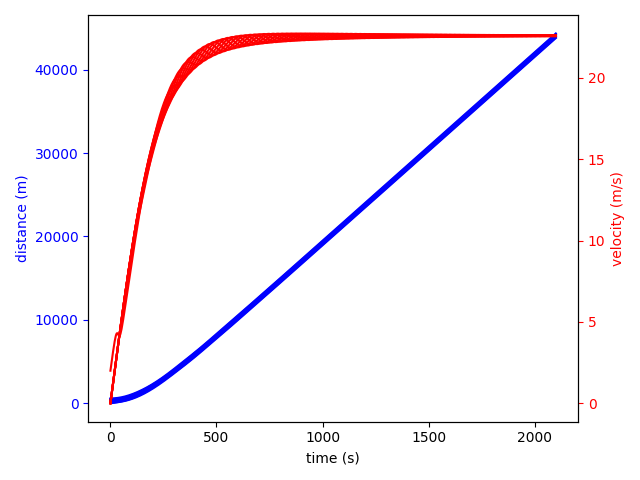
\includegraphics[scale = 0.5]{Figure_9.png}
			\captionof{figure}{Original setup with busses $(a = 0.1, b = 2, Nc = 6, Nb = 2)$}

			\indent While our inital acceleration and beginning velocity are undoubtedly worse than with a larger maximum acceleration, we can see that in terms of limiting behaviour that adding busses is overall about as effective
			as increasing our acceleration.

		\subsection*{Traffic Solutions Conclusions}

			\indent From these experiments run on our model we can take away several things. The number of vehicles on the road is the primary cause of traffic in our model, followed by human reaction time / acceleration
			time. Due to the nature of this system as a lot of coupled boxes, it really comes as no surprise that reducing the total number of vehicles through whatever means possible is our best bet (at least in this model)
			for reducing traffic. While this solution isn't perfect (not everyone will give up their cars and bus lines can be inflexible), it does highlight the shortcomings of a car only approach. We can also see that self driving cars (represented with better acceleration times) on their
			own are not a silver bullet for solving traffic, although they do contribute to improving it. They provide the best solution for mild congestion, but at most moderatly fix issues with major conjestion. However, even in a low conjestion setting we can see that replacing cars with busses is similar in efficacy to self driving cars.

			\indent In terms of more minor problems, this model also highlights that safer drivers on average contribute more to traffic. This suggests a potential sweet spot between safety and a driver's tendency to slam on their breaks. It would be tricky to find this though,
			as crashes are unaccounted for in this model while being a major contributor to traffic. Additionally, it shows that safety is a spot that self driving cars could potentially excel, as they are able to be more cautious with their braking while still improving traffic



	\end{multicols}


\end{document}
